%%
%% This is file `sample-sigconf.tex',
%% generated with the docstrip utility.
%%
%% The original source files were:
%%
%% samples.dtx  (with options: `sigconf')
%% 
%% IMPORTANT NOTICE:
%% 
%% For the copyright see the source file.
%% 
%% Any modified versions of this file must be renamed
%% with new filenames distinct from sample-sigconf.tex.
%% 
%% For distribution of the original source see the terms
%% for copying and modification in the file samples.dtx.
%% 
%% This generated file may be distributed as long as the
%% original source files, as listed above, are part of the
%% same distribution. (The sources need not necessarily be
%% in the same archive or directory.)
%%
%% The first command in your LaTeX source must be the \documentclass command.
\documentclass[sigconf]{acmart}
%%
%% \BibTeX command to typeset BibTeX logo in the docs
\AtBeginDocument{%
  \providecommand\BibTeX{{%
    \normalfont B\kern-0.5em{\scshape i\kern-0.25em b}\kern-0.8em\TeX}}}



%%
%% The majority of ACM publications use numbered citations and
%% references.  The command \citestyle{authoryear} switches to the
%% "author year" style.
%%
%% If you are preparing content for an event
%% sponsored by ACM SIGGRAPH, you must use the "author year" style of
%% citations and references.
%% Uncommenting
%% the next command will enable that style.
%%\citestyle{acmauthoryear}

%%
%% end of the preamble, start of the body of the document source.
\begin{document}

%%
%% The "title" command has an optional parameter,
%% allowing the author to define a "short title" to be used in page headers.
\title{Airborne Fluid Dynamic Simulator}

%%
%% The "author" command and its associated commands are used to define
%% the authors and their affiliations.
%% Of note is the shared affiliation of the first two authors, and the
%% "authornote" and "authornotemark" commands
%% used to denote shared contribution to the research.


\author{Kewei Sui}
\affiliation{%
 \institution{University of California, Berkeley}
 \city{Berkeley}
 \state{CA}
 \country{United States}}

\author{Xi Chen}
\affiliation{%
   \institution{University of California, Berkeley}
   \city{Berkeley}
   \state{CA}
   \country{United States}}

\author{Yitong Li}
\affiliation{%
 \institution{University of California, Berkeley}
 \city{Berkeley}
 \state{CA}
 \country{United States}}

%%
%% By default, the full list of authors will be used in the page
%% headers. Often, this list is too long, and will overlap
%% other information printed in the page headers. This command allows
%% the author to define a more concise list
%% of authors' names for this purpose.
\renewcommand{\shortauthors}{Sui and Chen and Li.}

%%
%% The abstract is a short summary of the work to be presented in the
%% article.
\begin{abstract}


  In early 2020, a novel and extremely contagious virus named Coronavirus-19 (Covid-19)  broke out worldwide. Research shows that the virus is mainly transmitted through droplets generated when an infected person coughs, sneezes, or exhales. 
  
 Here we implement an airborne fluid dynamics simulator that estimates the behavior of an in-compressible, homogeneous fluid under the Navier-Stokes equations that simulates virus transmission. Specifically, we simulate virus different spread paths by adjusting external factors such as velocity, pressure, temperature and density. This enables us to study how the virus reaches when people breath, sneeze and cough. 

\end{abstract}


%%
%% Keywords. The author(s) should pick words that accurately describe
%% the work being presented. Separate the keywords with commas.
\keywords{computer graphics, fluid dynamic simulation}

%% A "teaser" image appears between the author and affiliation
%% information and the body of the document, and typically spans the
%% page.
\begin{teaserfigure}
  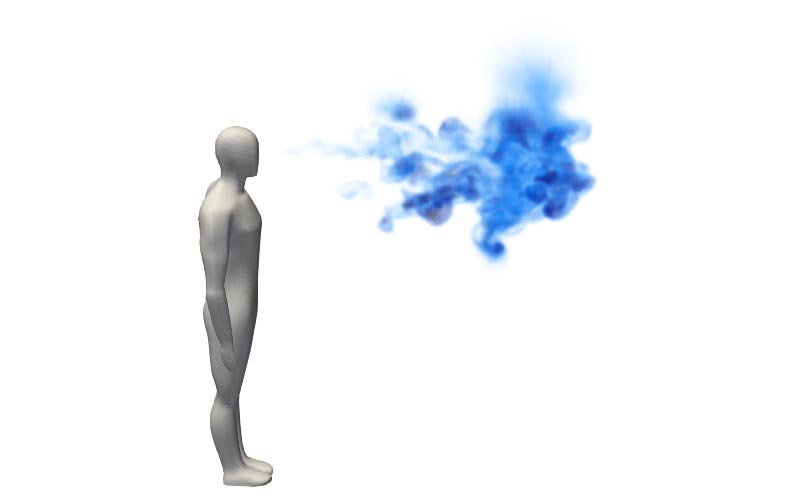
\includegraphics[width=\textwidth]{images/final.jpg}
  \caption{Airborne Transmission of Coronavirus\cite{figcite1}}
  \Description{Enjoying the baseball game from the third-base
  seats. Ichiro Suzuki preparing to bat.}
  \label{fig:teaser}
\end{teaserfigure}

%%
%% This command processes the author and affiliation and title
%% information and builds the first part of the formatted document.
\maketitle

\section{Introduction}
\subsection{Background}
The coronavirus COVID-19 is affecting 209 countries and territories around the world and two international conveyances. People in N.Y. and S.F. are forced to take shelter in place. Until April 9th, 14,802 people lost their lives because of this virus in the U.S., and 88,538 people died around the world. However, there are still many people who choose to neglect the existence of this dangerous virus and refuse to use face masks to protect themselves and other people. Thus, we wish to create a 2D fluid dynamics simulator to simulate the situations of people breathing, coughing, and sneezing. We hope to use this project to activate their awareness about how severe this disease is. It will be difficult to mimic the real dynamics for the spreading particles in these situations because of the complexity of the simulation. Thus, we will first implement a 2D fluid dynamics simulator based on Navier-Stokes equations and other reference projects. Then, we will try to utilize the actual data from researches about human coughs and sneezes for a real simulation.

\subsection{Goal}
Our goal of this project is to simulate the spread of particles in the air. We will then simulate if wearing masks makes any difference in the process of social networking. Hopefully, we could finally apply different materials on masks and simulate the positive effects of wearing masks against virus spreading.

The baseline of this project is to simulate the process of particle(virus) spreading. Through rendering fluid dynamics simulation, we will be able to see the virus' travelling path, velocity, and spreading time frame. In this part we will apply the Navier-Stokes equations and use GLSL fragment shaders to perform the physics calculations on the GPU.

If we get ahead of our schedule, we hope to simulate the fluid particles with some kind of barriers (to simulate masks). We would like to show the huge differences of particles' travelling path under situations with and without masks. We want to achieve this since ultimately we want to remind people of ways of protecting themselves from the Covid-19 virus and other airborne diseases.

We will measure our final result by both time and space complexity. We will also compare our fluids path with real-life airborne particle's travelling path to reveal the differences and consistencies. By the end of this project, we will be able to see the spreading paths of particles with different sizes in the air, we will also answer the ultimate question, that whether people should wear masks under airborne and direct contact diseases.

\section{Related Works}
\subsection{A study in droplet dispersion, heat and mass transfer}
 Aliabadi et al. developed a Computational Fluid Dynamics simulation of near-field cough and sneeze droplet dispersion and heat and mass transfer.\cite{Aliabadi} By considering various sources of variability in cough processes and ambient relative humidity, they simulated the motion of coughs in a quiescent background. They take humidity as a important factor since it affects the evaporation process and further affects the size of the droplets, which results in changes in vertical drop speed and axial penetration force.
\subsection{Cough simulators}
Zhang et al. established a Lagrangian model of droplet trajectories, and simulated cough in a predetermined ambient flow field.\cite{Zhang_2017} Parshina-Kottas et al creates a 3-D simulation of cough spreading using research data from the Kyoto Institute of Technology by computing the movements and separation of various sizes of droplets produced by coughs.\cite{Parshina-Kottas}


\section{Our work}

To simulate the behavior of fluids, we need to find a way to represent the physical properties at a certain time spot. We used 2D fields to represent the various velocity,temperature and density at different positions in the grid. After locating the fluids, We applied Navier-Stokes Equations in our calculation of forces, velocity, density, pressure. Combining these factors together gives us a complete simulation of fluid particles transmitting in the air.

\subsection{Navier-Stokes Equations}
Navier-Stokes Equations is used to describe the motion of incompressible and homogeneous fluid.
\begin{equation}
\frac{\partial u}{\partial t} = -(u \cdot \nabla)u - \frac{1}{\rho} \nabla p + v \nabla ^2 u + F
\end{equation}


\subsection{Advection}
The first term in equation 1 represents the advection field along the fluid's velocity field. Since the velocity causes the fluid to transport particles with the flow, we need to constantly use this term to update not only velocity, but also density and temperature which is affected by changes in velocity. 

\subsection{Pressure}
The second term in equation 1 represents the pressure of fluids, which is calculated as force per unit area. We keep track of pressure because particles of a fluid move around each other, once adding force to one part, other parts of particles would also got "squished". Specifically, we used the Poisson Equation to solve for pressure. 

\subsection{Diffusion}
The third term in equation 1 is named viscosity, which is a measure of how resisting a fluid is to flow. Since we are simulating particles in air where viscosity is virtually zero, we do not considerate viscosity and left it out of our implementation. 

\subsection{External Forces}
The fourth term encapsulates acceleration due to external forces applied to the fluid. In our case, it refers to the (in most cases, horizontal) force where human sneezes the particles out of their mouths. During the transmission paths, gravity and buoyancy also count as external forces in the vertical direction. 


\begin{figure}[!htbp]
\centering
        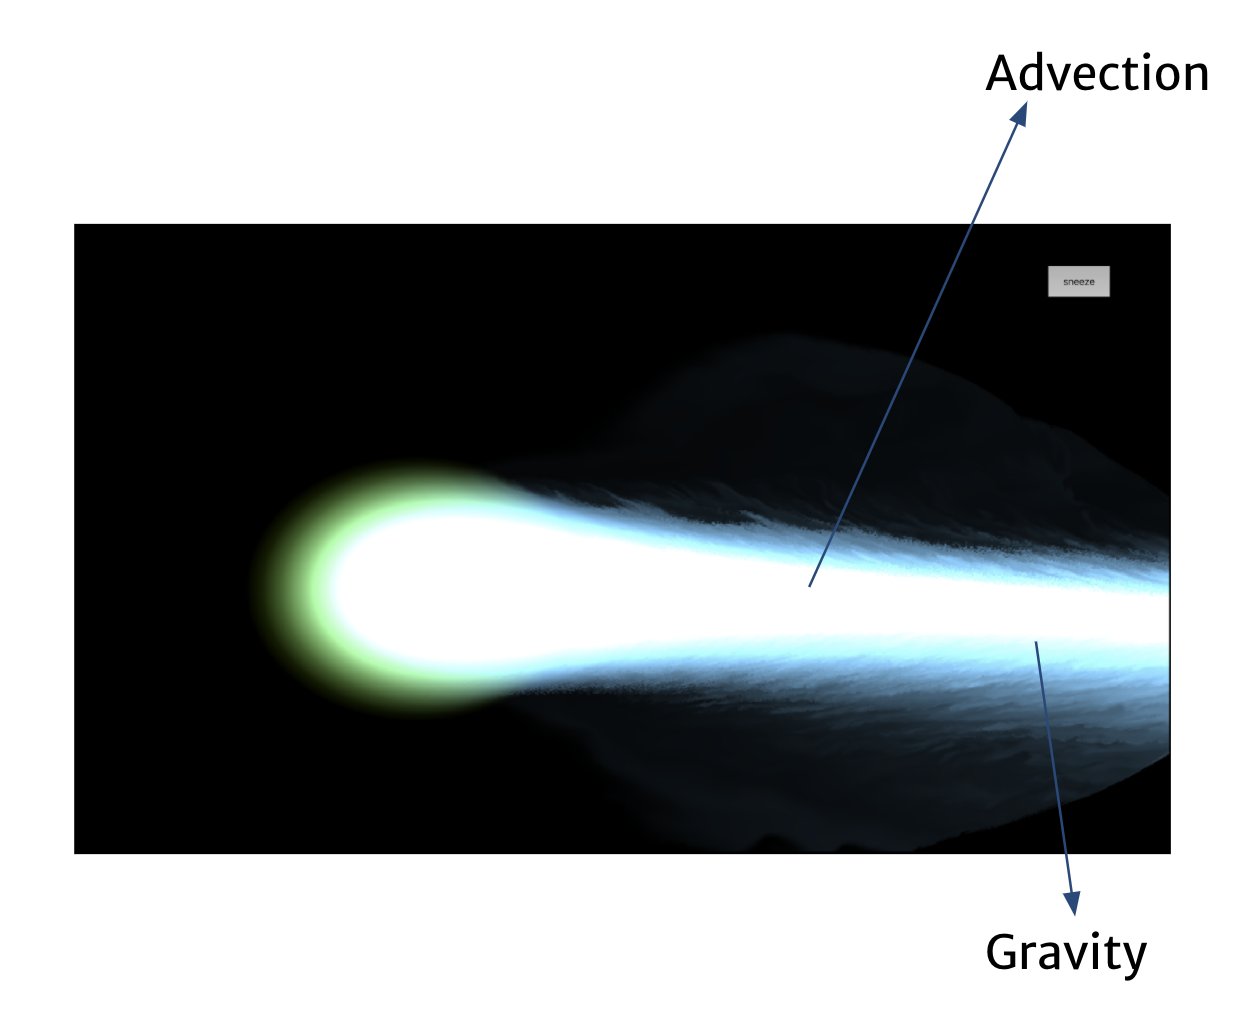
\includegraphics[width=\linewidth]{images/simulation1.png}
    \caption{Our simulation of advection and gravity}
    \label{fig:verticalcell}
\bigbreak
\centering
        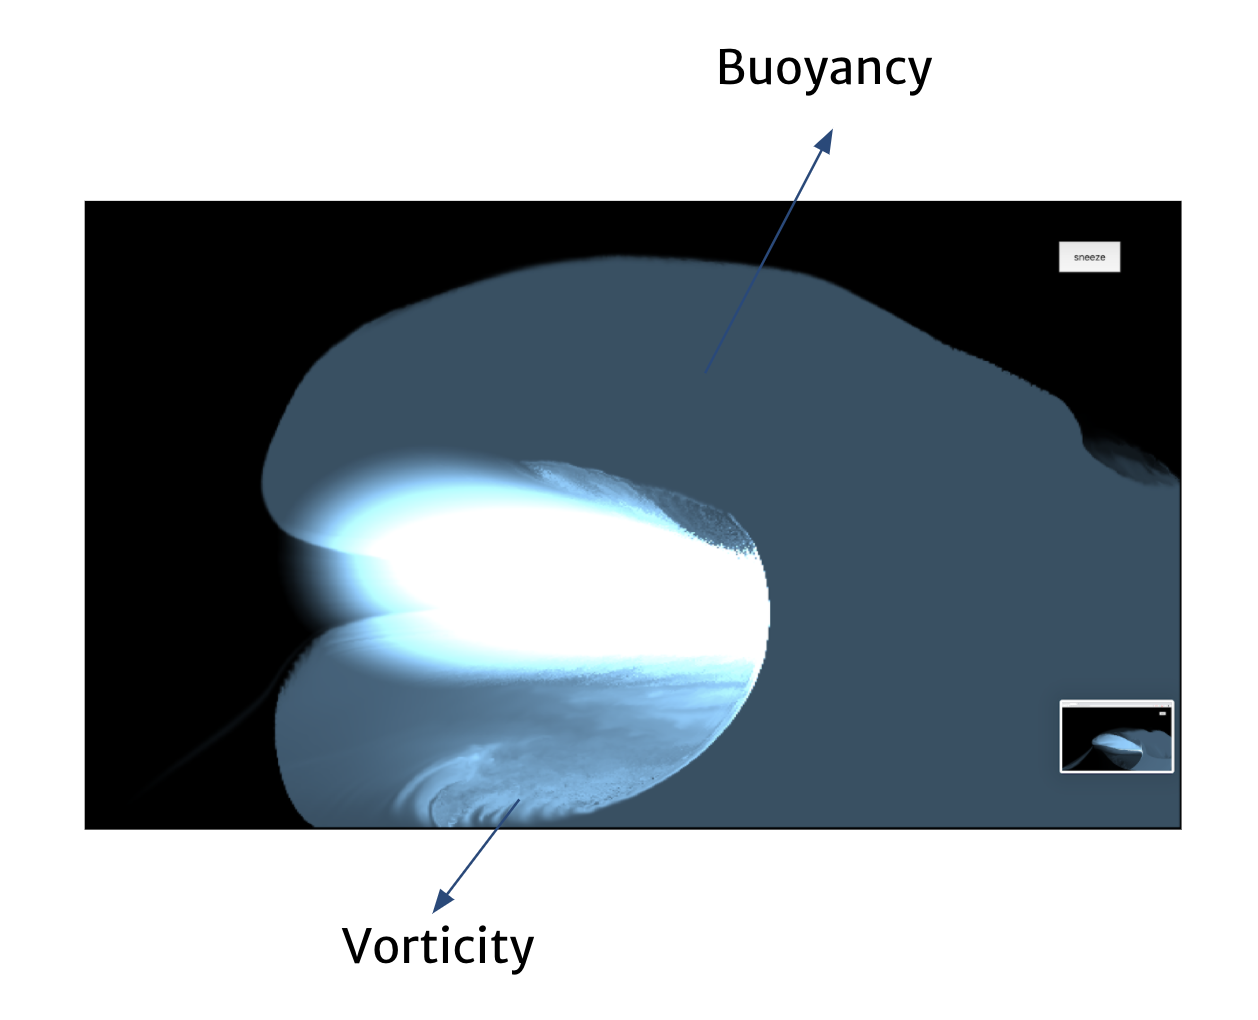
\includegraphics[width=\linewidth]{images/simulation2.png}
    \caption{Our simulation of vorticity and buoyancy}
    \label{fig:verticalcell}
\end{figure}


%%
%% The next two lines define the bibliography style to be used, and
%% the bibliography file.
\newpage
\bibliographystyle{ACM-Reference-Format}
\bibliography{sample-base}

\end{document}
\endinput
%%
%% End of file `sample-sigconf.tex'.
